\section{Requirement analysis} \label{ch:req}
This section will analyze the requirements of the re-entry mission. It will start by providing a requirements discovery tree, which visualizes the way the different requirements on the re-entry vehicle flow down from the top level mission requirements and constraints. This will be followed by an analysis of the subsystem requirements. This analysis will follow from the flown down presented in the \gls{rdt}. Finally, the requirements will be as precisely defined and documented as possible at this stage. For the unknown values the acronym \gls{tbd} will be used. The output of this final step will be the requirements used during the product design. %Guido: Dit moet nog beter geformuleerd worden, maar kon even niets beters bedenken

\subsection{Requirements Discovery Tree}
The overarching mission requires the system to perform a manned re-entry on Mars. Several performance requirements and mission constraints are imposed on the system. These overall requirements and constraints were detailed in the project plan \cite{Balasooriyan2015}. From these overall requirements and constraints, subsystem requirements can be derived. Figure \ref{fig:RBS} graphically displays this requirements discovery, and provides a sample parameter which has a requirement imposed on it due to the top level requirements. Each of the subsystems' requirements will be elaborated and expanded upon in the remainder op this section. 


\vspace{-5mm}
\begin{figure}[H]
\centering
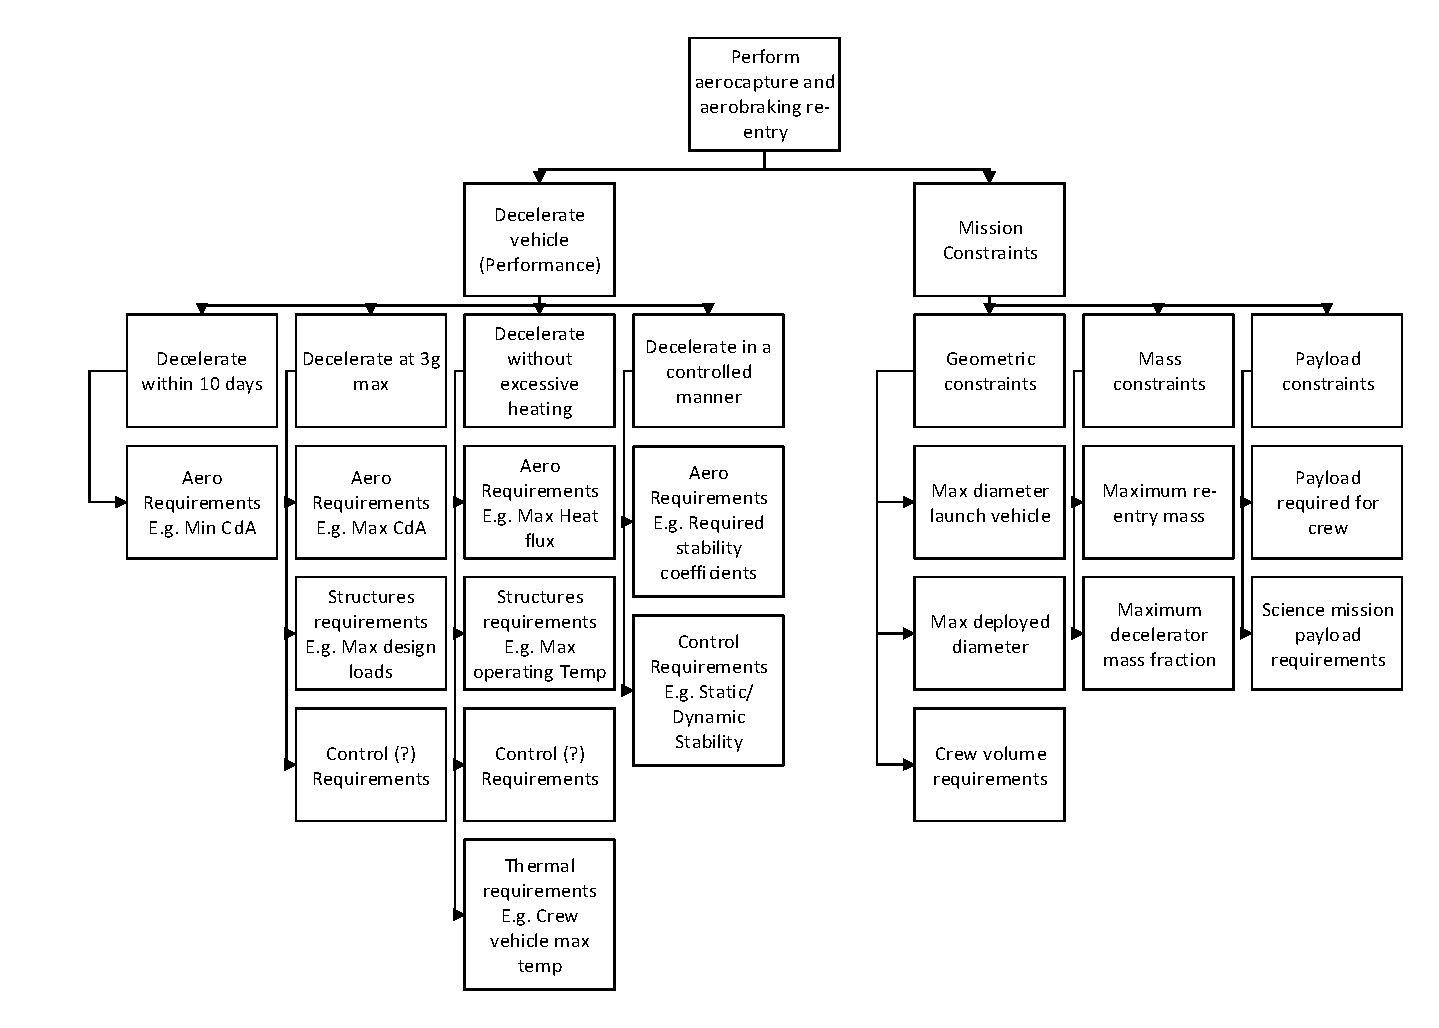
\includegraphics[width=1.00\textwidth]{Figure/RBS.pdf}
\vspace{-5mm}
\caption{Requirements Discovery Tree} 
\label{fig:RBS}
\end{figure}


\subsection{Top-level requirements}
The requirement discovery tree is used to formulate the high level mission requirements. These requirements are then used to derive further system and subsystem requirements in subsequent sessions. The high level requirements are presented in table \ref{tab:toplevelreq}.

\begin{table}[H]
	\caption{Overview of high level mission requirements} \label{tab:toplevelreq}
	\begin{tabular}{|p{0.20\textwidth}|p{0.7\textwidth}|}
    \hline
    ID          & Description                                                                                                      \\ \hline \hline
    CIA-A01 & The re-entry vehicle shall decelerate from a velocity of $7kms^-1$ \\ \hline
    CIA-A02 & The re-entry vehicle shall operate within mission constraints                                               \\ \hline
    CIA-A01-01 & The re-entry vehicle shall decelerate to a velocity of \gls{tbd}     \\ \hline
    CIA-A01-02 & The re-entry vehicle shall not exert an acceleration greater than $29.4 m/s^-2	$ on any crew member for the duration of the mission			\\ \hline
    CIA-A01-03 & The re-entry vehicle shall not be heated excessively  \\ \hline
    CIA-A01-04 & The re-entry vehicle shall be in a controlled state for the duration of the mission                            \\ \hline
    CIA-A02-01 & The re-entry vehicle shall meet all geometric constraints imposed by the mission                           \\ \hline
    CIA-A02-02 & The re-entry vehicle shall meet all mass constraints imposed by the mission                                      \\ \hline
	CIA-A02-03 & The re-entry vehicle shall meet all payload constraints imposed by the mission \\ \hline
	CIA-A01-01-01 & The re-entry vehicle shall reach its final velocity at an altitude of \gls{tbd} m \\ \hline
	CIA-A01-01-02 & The re-entry vehicle shall reach its final velocity within 10 days of mission start \\ \hline
    \end{tabular}
\end{table}

\subsection{Aerodynamic Requirements Discovery} 
\label{sec:aero}
A number of aerodynamic requirements can be seen in figure \ref{fig:RBS}. These will all be discussed here and have been summarized in table \ref{tab:aeroreqs}. 


\begin{table}[h]
	\caption{Overview of Aerodynamic requirements}
	\label{tab:aeroreqs}
	\begin{tabular}{|p{0.2\textwidth}|p{0.7\textwidth}|}
		\hline
		ID & Description \\
		\hline \hline
		CIA-B01-Aero-01 & The system shall produce a maximum heat flux of no more than TBD [$\frac{W}{cm^{2}}$] \\ \hline
		CIA-B07-Aero-01 & The system shall have a \gls{sym:CD}\gls{sym:A} of TBD $m^{2}$ \\ \hline
	\end{tabular}
\end{table}

Requirement CIA-B01-Aero-01 follows from the entry velocity of 7 [$\frac{km}{s}$]. Since the heat flux subjected upon a body is proportional to $\gls{sym:V}^{3}$ \cite{Tauber1986} the highest values for the heat flux will be found during the first orbit around Mars. 
Requirement CIA-B07-Aero-01 is caused by the need for a limitation of the maximum allowable decelerations that occur. This can have a significant impact on the mission and mission duration, since this limits the maximum allowable drag force that can be achieved.
\subsection{Structural Requirements Discovery} \label{sec:struct}
The vehicle structure faces a number of requirements, functional and operational. The functional requirements are stated in Table \ref{tab:strucfuncrequirements}, the operational requirements in Table \ref{tab:strucoprequirements}. These requirements are briefly discussed hereafter.
\begin{table}[H]
	\caption{Overview of functional requirements on structures subsystem}
	\begin{tabular}{|p{0.20\textwidth}|p{0.70\textwidth}|}
    \hline
    ID          & Description                                                                                                      \\ \hline \hline
    CIA-B01-Struc-01 & The structure shall operate within a temperature range of [\gls{tbd},\gls{tbd}] degrees Celsius           \\ \hline
    CIA-B02-Struc-02 & The structure shall support deployment \\ \hline
    CIA-B07-Struc-03 & The structure shall sustain the maximum mechanical loads without failure                           \\ \hline
    CIA-B09-Struc-04 & The structure shall connect payload and deceleration mechanism \\ \hline
    \end{tabular}
    \label{tab:strucfuncrequirements}
\end{table}
Requirement CIA-B01-Struc-01 follows from the aerodynamic heating as a consequence of the dissipation of kinetic energy corresponding to a velocity of 7 [km/s], as stated in requirement CIA-A01. The \gls{tps} reduces the temperature to within acceptable limits, which are translated to a range of temperature in which the structures subsystem should operate. These temperatures therefore follow from the \gls{tps}. This requirement is essential because temperature can have a substantial effect on the mechanical properties of materials as well as thermal expansion \cite{Callister2007}. These mechanical properties are essential to meet requirement CIA-B07-Struc-03, namely to handle the structural loads induced during aerocapture and (re-)entry. These have been limited to 3g in each axis in requirement CIA-A03. In addition, if a deployment functionality  (for example an inflation system) is a concept feature, deployment should be performed by the subsystem; in case such a functionality is not present, there is no deployment, hence nothing to support and the requirement is logically satisfied. This is stated in requirement CIA-B02-Struc-02. Lastly, payload and deceleration mechanism should be connected to prevent separation during re-entry and satisfy the payload constraint. This is stated in requirement CIA-B09-Struc-04.

\begin{table}[H]
	\caption{Overview of operational requirements on structures subsystem}
	\begin{tabular}{|p{0.20\textwidth}|p{0.70\textwidth}|}
    \hline
    ID          & Description                                                                                                      \\ \hline \hline
    CIA-B02-Struc-05 & The structure shall have a maximum diameter not exceeding 12 [m] in deployed configuration     \\ \hline
    CIA-B03-Struc-06 &  The structure shall have a maximum diameter not exceeding 5 [m] in stowed configuration                              \\ \hline
    CIA-B04-Struc-07 & The structure shall have a mass not exceeding 350 [kg]\\ \hline
    \end{tabular}
    \label{tab:strucoprequirements}
\end{table}
The operational requirements CIA-B02-Struc-05 and CIA-B03-Struc-06 follow from the geometric constraints (by launcher considerations). Requirement CIA-B04 states that the structural subsystem should respect the mass budget.
\subsection{Thermal Requirements Discovery} \label{sec:therm}
The requirements for the thermal subsystem flow down from the \gls{rdt} and are listed in Table \ref{tab:thermalreq}. The requirements are split up in two parts, the \gls{tps} and the \gls{tcs}. The \gls{tps} mainly distributes the heat load and flux generated by decelerating the re-entry vehicle, whereas the \gls{tcs} controls the temperature of the payload and other subsystems.


\begin{table}[H]
	\caption{Overview of thermal requirements}
	\begin{tabular}{|p{0.2\textwidth}|p{0.70\textwidth}|}
    \hline
    ID          & Description                                                                                                      \\ \hline \hline
   CIA-Func-B03-TPS-01 & The TPS shall be able to withstand the maximum heat flux of \gls{tbd} $ \left[\frac{W}{cm^2}\right] $               
\\ \hline
    CIA-Func-B03-TPS-02 &  The TPS shall be able to withstand the maximum heat load of \gls{tbd} $ \left[\frac{J}{cm^2}\right] $               
\\ \hline
    CIA-Func-B03-TCS-01 & The TCS shall keep the subsystems within their operative temperature range                                            
\\ \hline
    CIA-Func-B03-TCS-02-crewmodule & The TCS shall keep the crew module within a temperature range of \gls{tbd} and \gls{tbd} $ \left[^{\circ}C\right] $                                        
\\ \hline
    CIA-Func-B03-TCS-03-structure & The TCS shall keep the structure module within a temperature range of \gls{tbd} and \gls{tbd} $ \left[^{\circ}C\right] $                                        
\\ \hline
	CIA-Op-B03-Therm-01 	&	The thermal system shall have a mass not exceeding 500 [kg]  							\\ \hline
    \end{tabular}
    \label{tab:thermalreq}
\end{table}

Requirement IA-Func-B03-TPS-01 follows from the trajectory the re-entry vehicle is following and is bounded by the shortest trajectory, the maximum undershoot trajectory, the vehicle can follow. During this trajectory the vehicle will see the fastest heat development. Not only the fastest heat development is important, but also the duration of deceleration. For the longest trajectory, the maximum overshoot trajectory, energy will be dissipated into the shell. The \gls{tps} should be able to cope with this heat development over time. This need is covered by requirement  CIA-Func-B03-TPS-02. The payload and subsystems are only able to withstand a certain temperature range. To keep the payload and subsystems within this range the \gls{tcs} follows requirement CIA-Func-B03-TCS-01. For now the structure and crew module have been explicitly listed, however it is expected that more subsystems will be added to the requirements further on in the design process.


\subsection{Control}

**Intro**

\subsubsection{Assumptions}

**Primary and Secondary assumptions**

\subsubsection{Trim point}

**Moment equilibrium figures/equations**
**CG-location plot(s)  with conclusion on CG for AoA~20 and sideslip angle=0**

\subsubsection{Stability}

**From E.Mooij**

\subsubsection{Available control systems}

**Intro**

\paragraph{\acrfull{cg} offset}

**Not nessesary for AoA, not feasible for sideslip**

\paragraph{Thrusters}

**Sebstiaan**

\paragraph{Aerodynamic surfaces}

**Guido**




\subsection{Control Requirements Discovery} \label{sec:req-orbit}
\subsection{Mission Constraints} \label{sec:MisCon}
\begin{table}[H]
	\caption{Overview of Mission Constraints}
	\begin{tabular}{|p{0.10\textwidth}|p{0.85\textwidth}|}
    \hline
    ID          & Description                                                                                                      \\ \hline \hline
		CIA-A02-01-01 & The reentry vehicle shall have an undeployed diameter smaller than 5m                         				            \\ \hline
		CIA-A02-01-02 & The reentry vehicle shall have a deployed diameter smaller than 12m                         				            \\ \hline
		CIA-A02-01-03 & The reentry vehicle shall have a volume capable of accommodating 6 crew members                        				            \\ \hline
		CIA-A02-02-01 & The reentry vehicle shall have a mass of 10000 kg at the start of the re-entry                       				            \\ \hline
		CIA-A02-03-01 & The reentry vehicle shall carry sufficient provisions for the crew for the duration of the mission
		CIA-A02-03-02 & The reentry vehicle shall be able to carry the mission payload								\\ \hline
		CIA-B02-02-02-01 & The Hypersonic decelerator shall have a mass fraction of no greater than 10\% of the vehicle mass  \\ \hline
		CIA-B02-02-02-02 & The Crew module shall have a mass fraction of no greater than 90\% of the vehcile mass \\ \hline
		
		\end{tabular}
    \label{tab:MissionCon}
\end{table}




